\documentclass[14pt,aspectratio=169]{beamer}
\usetheme{Marburg}
\usefonttheme{professionalfonts}
\usepackage[utf8]{inputenc}
\usepackage{scalerel}
\usepackage[T1]{fontenc}
\usepackage{amsmath, amssymb}
\usepackage{amsfonts}
\usepackage{graphicx}
\DeclareUnicodeCharacter{2212}{-}

\newcommand{\TT}{Forecasting Stock Price Using Sentiment Analysis and LSTM Networks}
\newcommand{\IN}{Introduction}
\newcommand{\WF}{Workflow}
\newcommand{\DAT}{Data Description}
\newcommand{\ALG}{Main Models}
\newcommand{\THE}{Theory}
\newcommand{\IMP}{Implementation}
\newcommand{\CC}{Conclusion}
\newcommand{\XL}{XLNet}
\newcommand{\LS}{LSTM}
\newcommand{\MM}{Main Model}
\newcommand{\SC}{Source}
\newcommand{\PRD}{Prediction}
\newcommand{\PE}{Performance Evaluation}
\newcommand{\XLI}{XLNet Implementation}

\author{Blake Hillier, Grace Li, Joe Puhalla}

\title{\TT}
%\setbeamercovered{transparent} 
\setbeamertemplate{navigation symbols}{}
\date{5 May 2020} 
\subject{Advanced Big Data Analysis} 
\begin{document}

\begin{frame}
\titlepage
\end{frame}

\begin{frame}{Outline}
    \tableofcontents
\end{frame}

\section{\IN}
\begin{frame}{\IN}
\begin{itemize}
    \item Forecasting stock prices is a widely known problem many people have attempted to solve through various models. \\
    \item We propose a model using macro-economic variables to predict the future price of a stock, one of which is statements from the Federal Reserve about decisions on economic policies.\\
    \item Our model is comprised of XLNet to perform sentiment analysis on one macro-economic variable and an LSTM Neural Network to combine all the variables while capturing the effect time has on the future stock price.
\end{itemize}
\end{frame}

\subsection{\WF}
\begin{frame}{\WF}
\begin{figure}
    \centering
    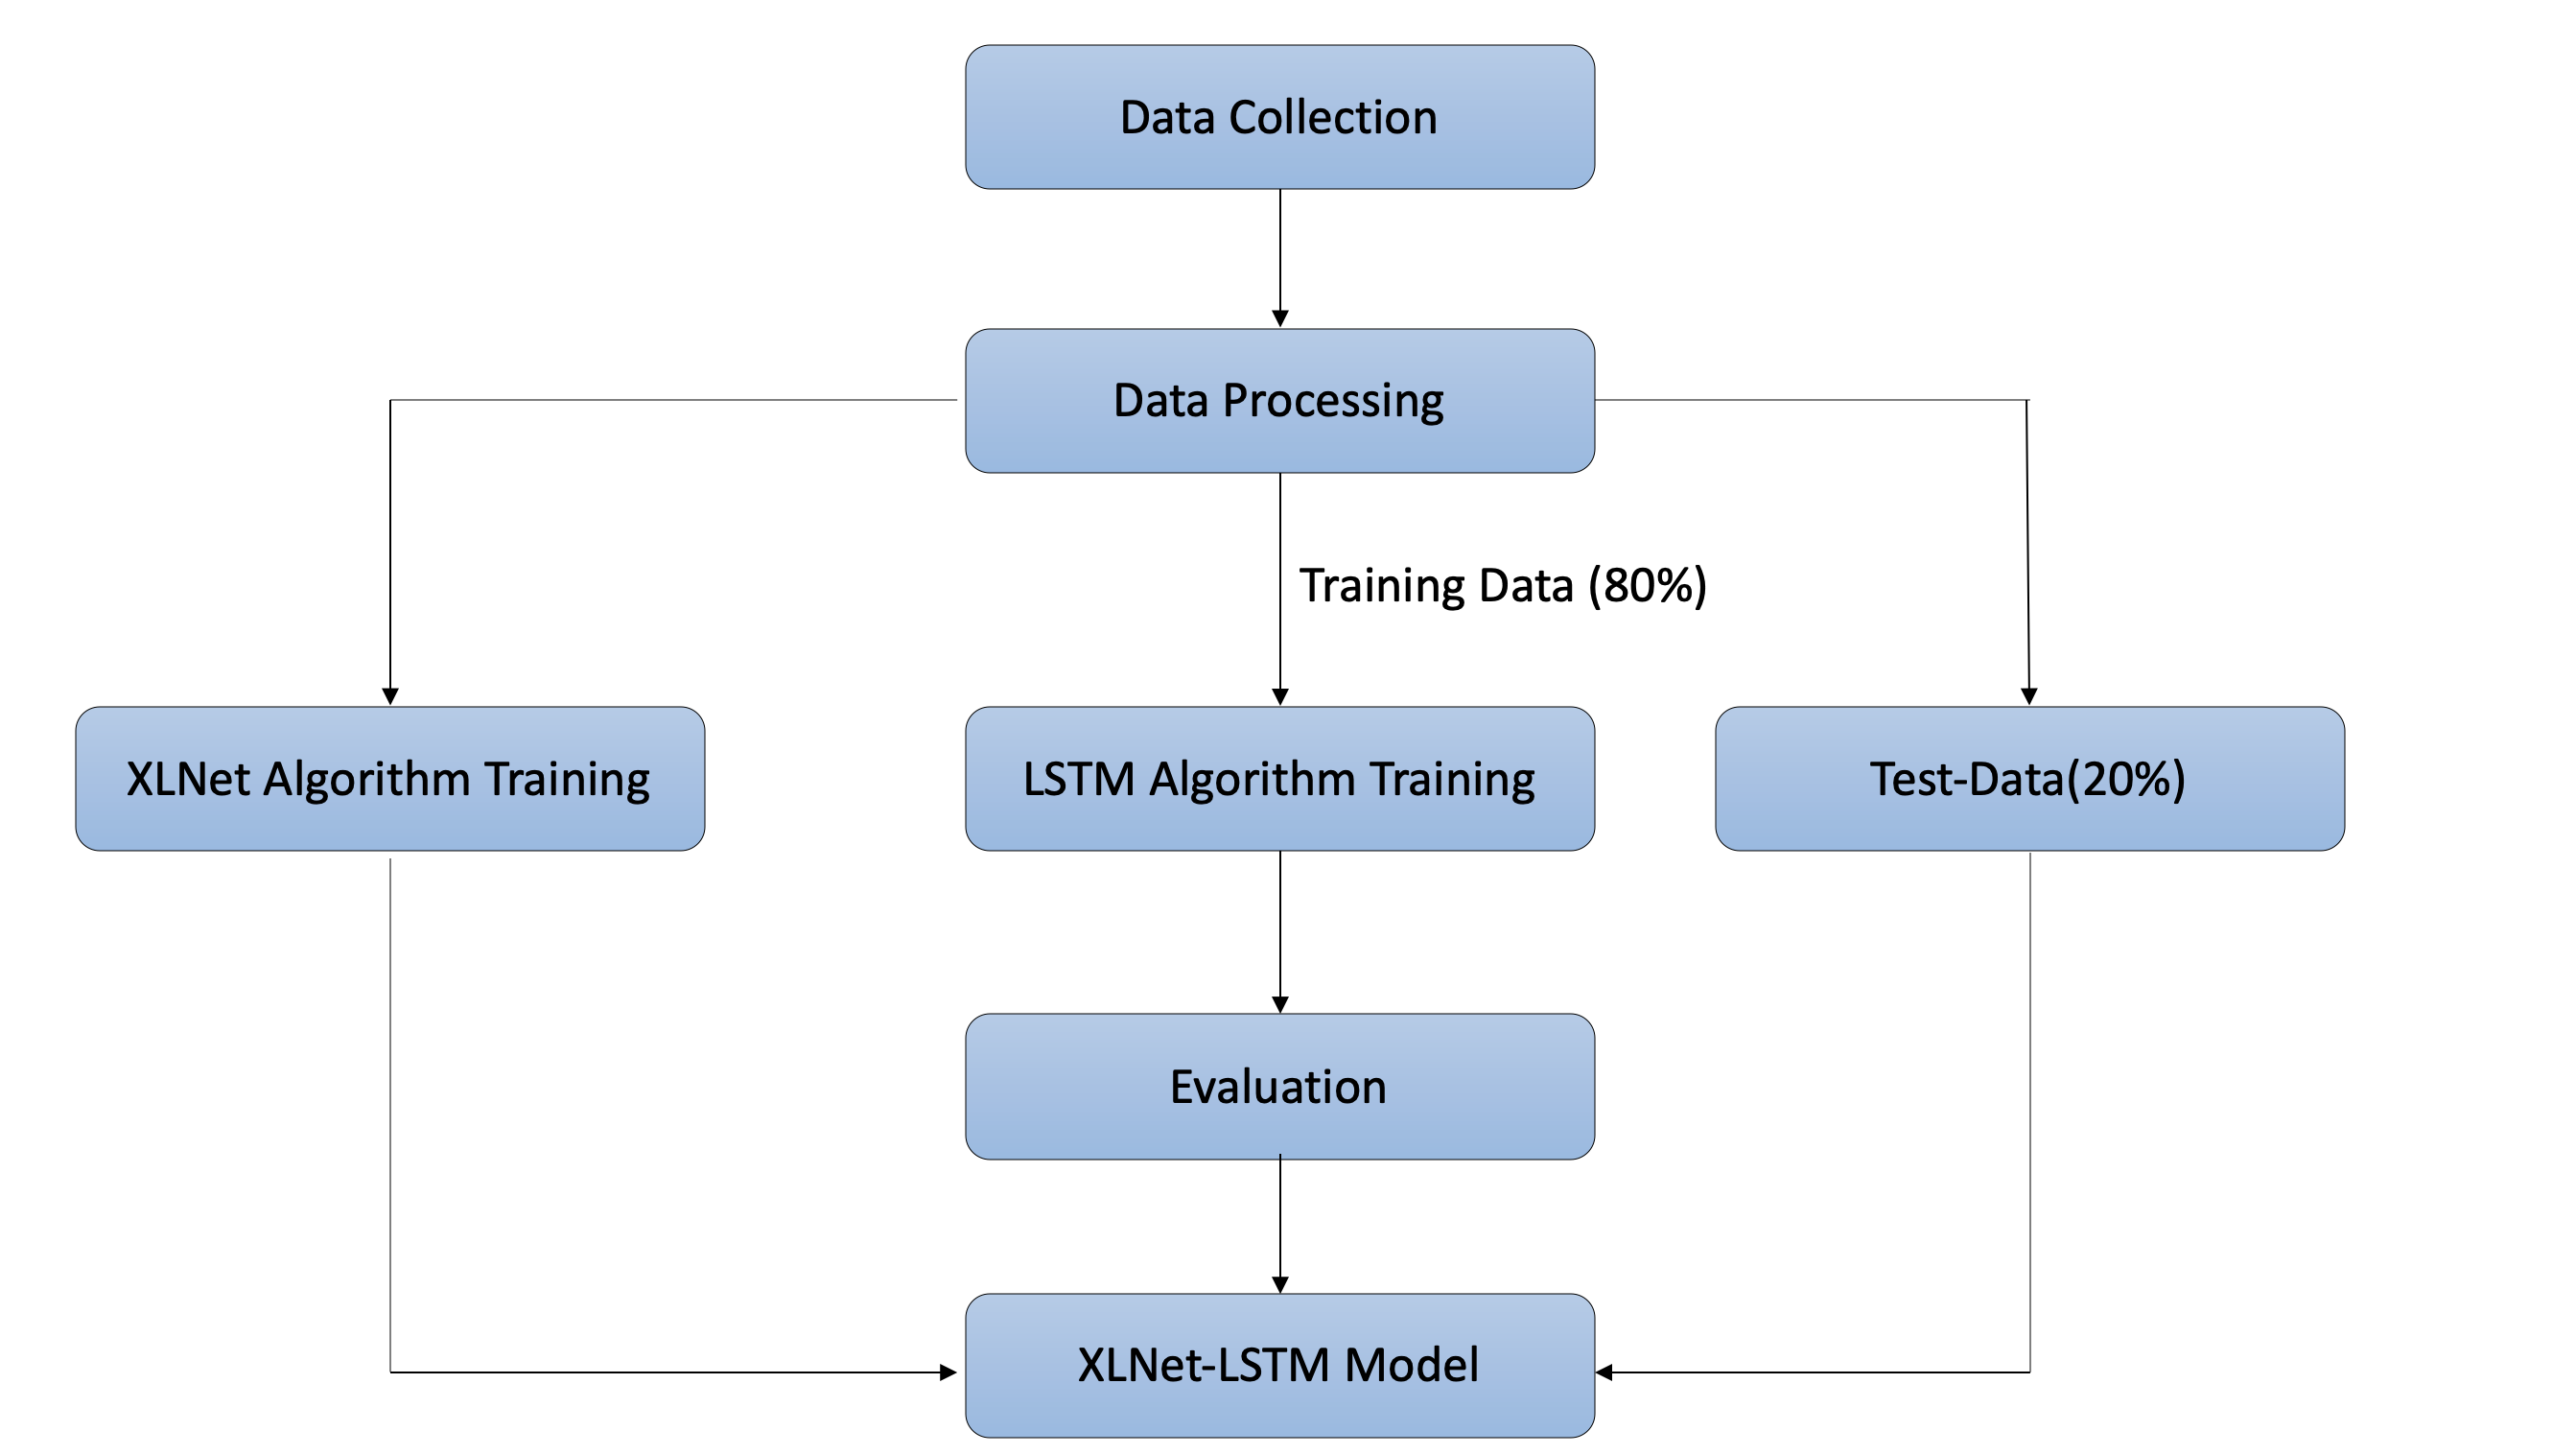
\includegraphics[width=11cm]{workflow_.png}
    \caption{Workflow}
    \label{fig:my_label}
\end{figure}
\end{frame}

\subsection{\DAT}
\begin{frame}{\DAT}
\begin{figure}
    \centering
    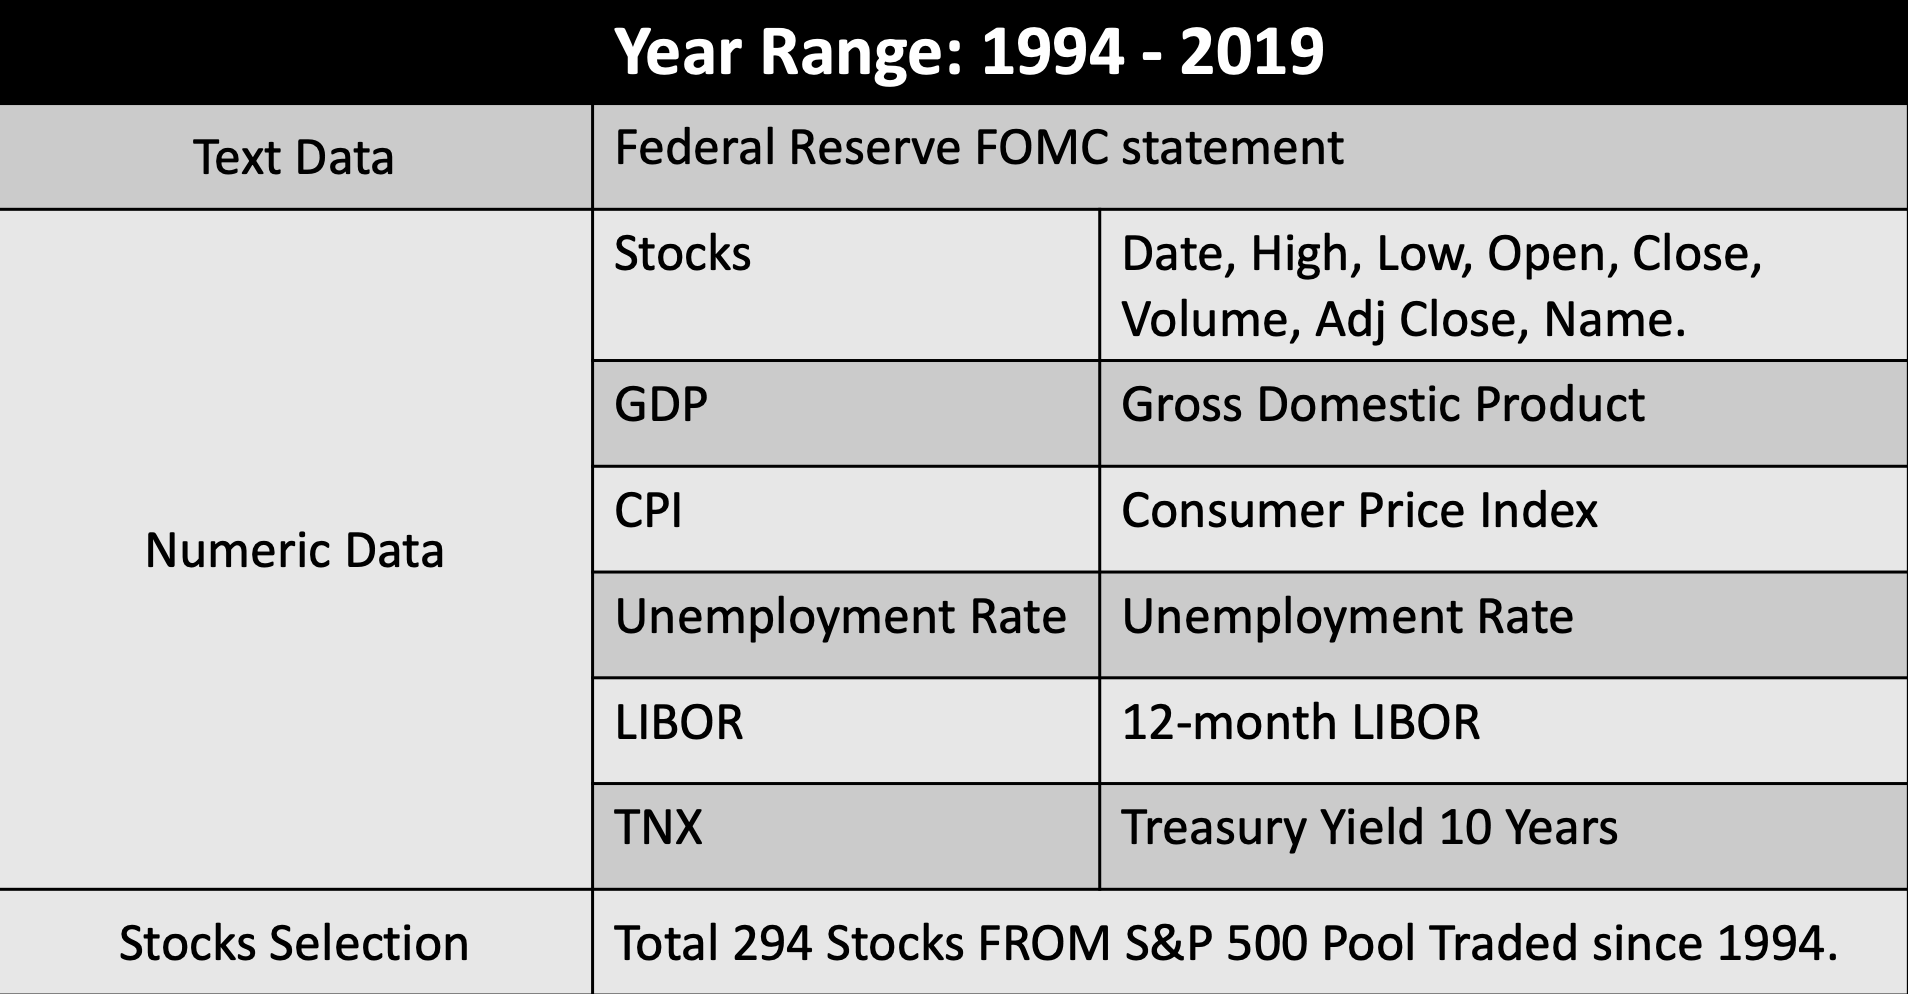
\includegraphics[width=10cm]{Notes/DataList.png}
    \caption{Data Description}
    \label{fig:my_label}
\end{figure}
\end{frame}

\subsection{\PE}
\begin{frame}{\PE}
We validated our XLNet-LSTM based on the S&P 500 stocks. We calculate the Mean Absolute Error (MAE) to evaluate the proposed methods, which is defined as
$$ MAE_{t} = \frac{1}{L} \sum_{i=1}^{L} \frac{\sum_{i=1}^{n} \mid y_{i, t} - x_{i, t} \mid }{n} = \frac{1}{L} \sum_{i=1}^{L} \frac{\sum_{i=1}^{n} \mid e_{i, t} \mid}{n}$$
Where $y_{i, t}$ is the real stock price of the $i$-th stock on the $t$-th day, $L$ is the number of stocks and $x_{i,t}$ is the corresponding prediction result. 
\end{frame}

\section{\XL}
\subsection{\THE}
\begin{frame}{\XL}
    XLNet is an autoregressive pretraining approach for NLP models which solves: \scalebox{0.85}{\begin{equation*}
        \max_{\theta}E_{z\sim Z_{T}}\left[\sum_{t=1}^{T}\log p_{\theta}(x_{z_{t}}|x_{z<t})\right]=E_{z\sim Z_{T}}\left[\sum_{t=1}^{T}\log\frac{e^{g_{\theta}(x_{z<t,z_{t}})l(x_{t}})}{\sum_{x^{'}}e^{g_{\theta}(x_{z<t,z_{t}})l(x^{'})}}\right]
    \end{equation*}} where \begin{itemize}
        \item $Z_{T}$ is the set of all permutations of text of length $T$ \\
        \item $z\in Z_{T}, x_{z<t}$ is the sequence of text from 1 to $t−1$ \\
        \item $g_{\theta}$ transforms $x$ to a sequence of hidden words with the first $t-1$ set of words as additional information
    \end{itemize}
    \textbf{Note: $g_{\theta}$ permutes $x$ and then masks the words}
\end{frame}


\subsection{\IMP}
\begin{frame}{\XL}
    We used pytorch's implementation of XLNet-base for our model.
    \begin{itemize}
        \item Sentiment was assigned to the Fed's Statements by looking at the percent change of various macro variables
        \item We used an 80/20 Train/Test split \\
        \item Testing was done using a GPU on Colab
    \end{itemize}
\end{frame}

\begin{frame}
    \vspace{-0.55in}
    \begin{figure}[ht]
        \centering
        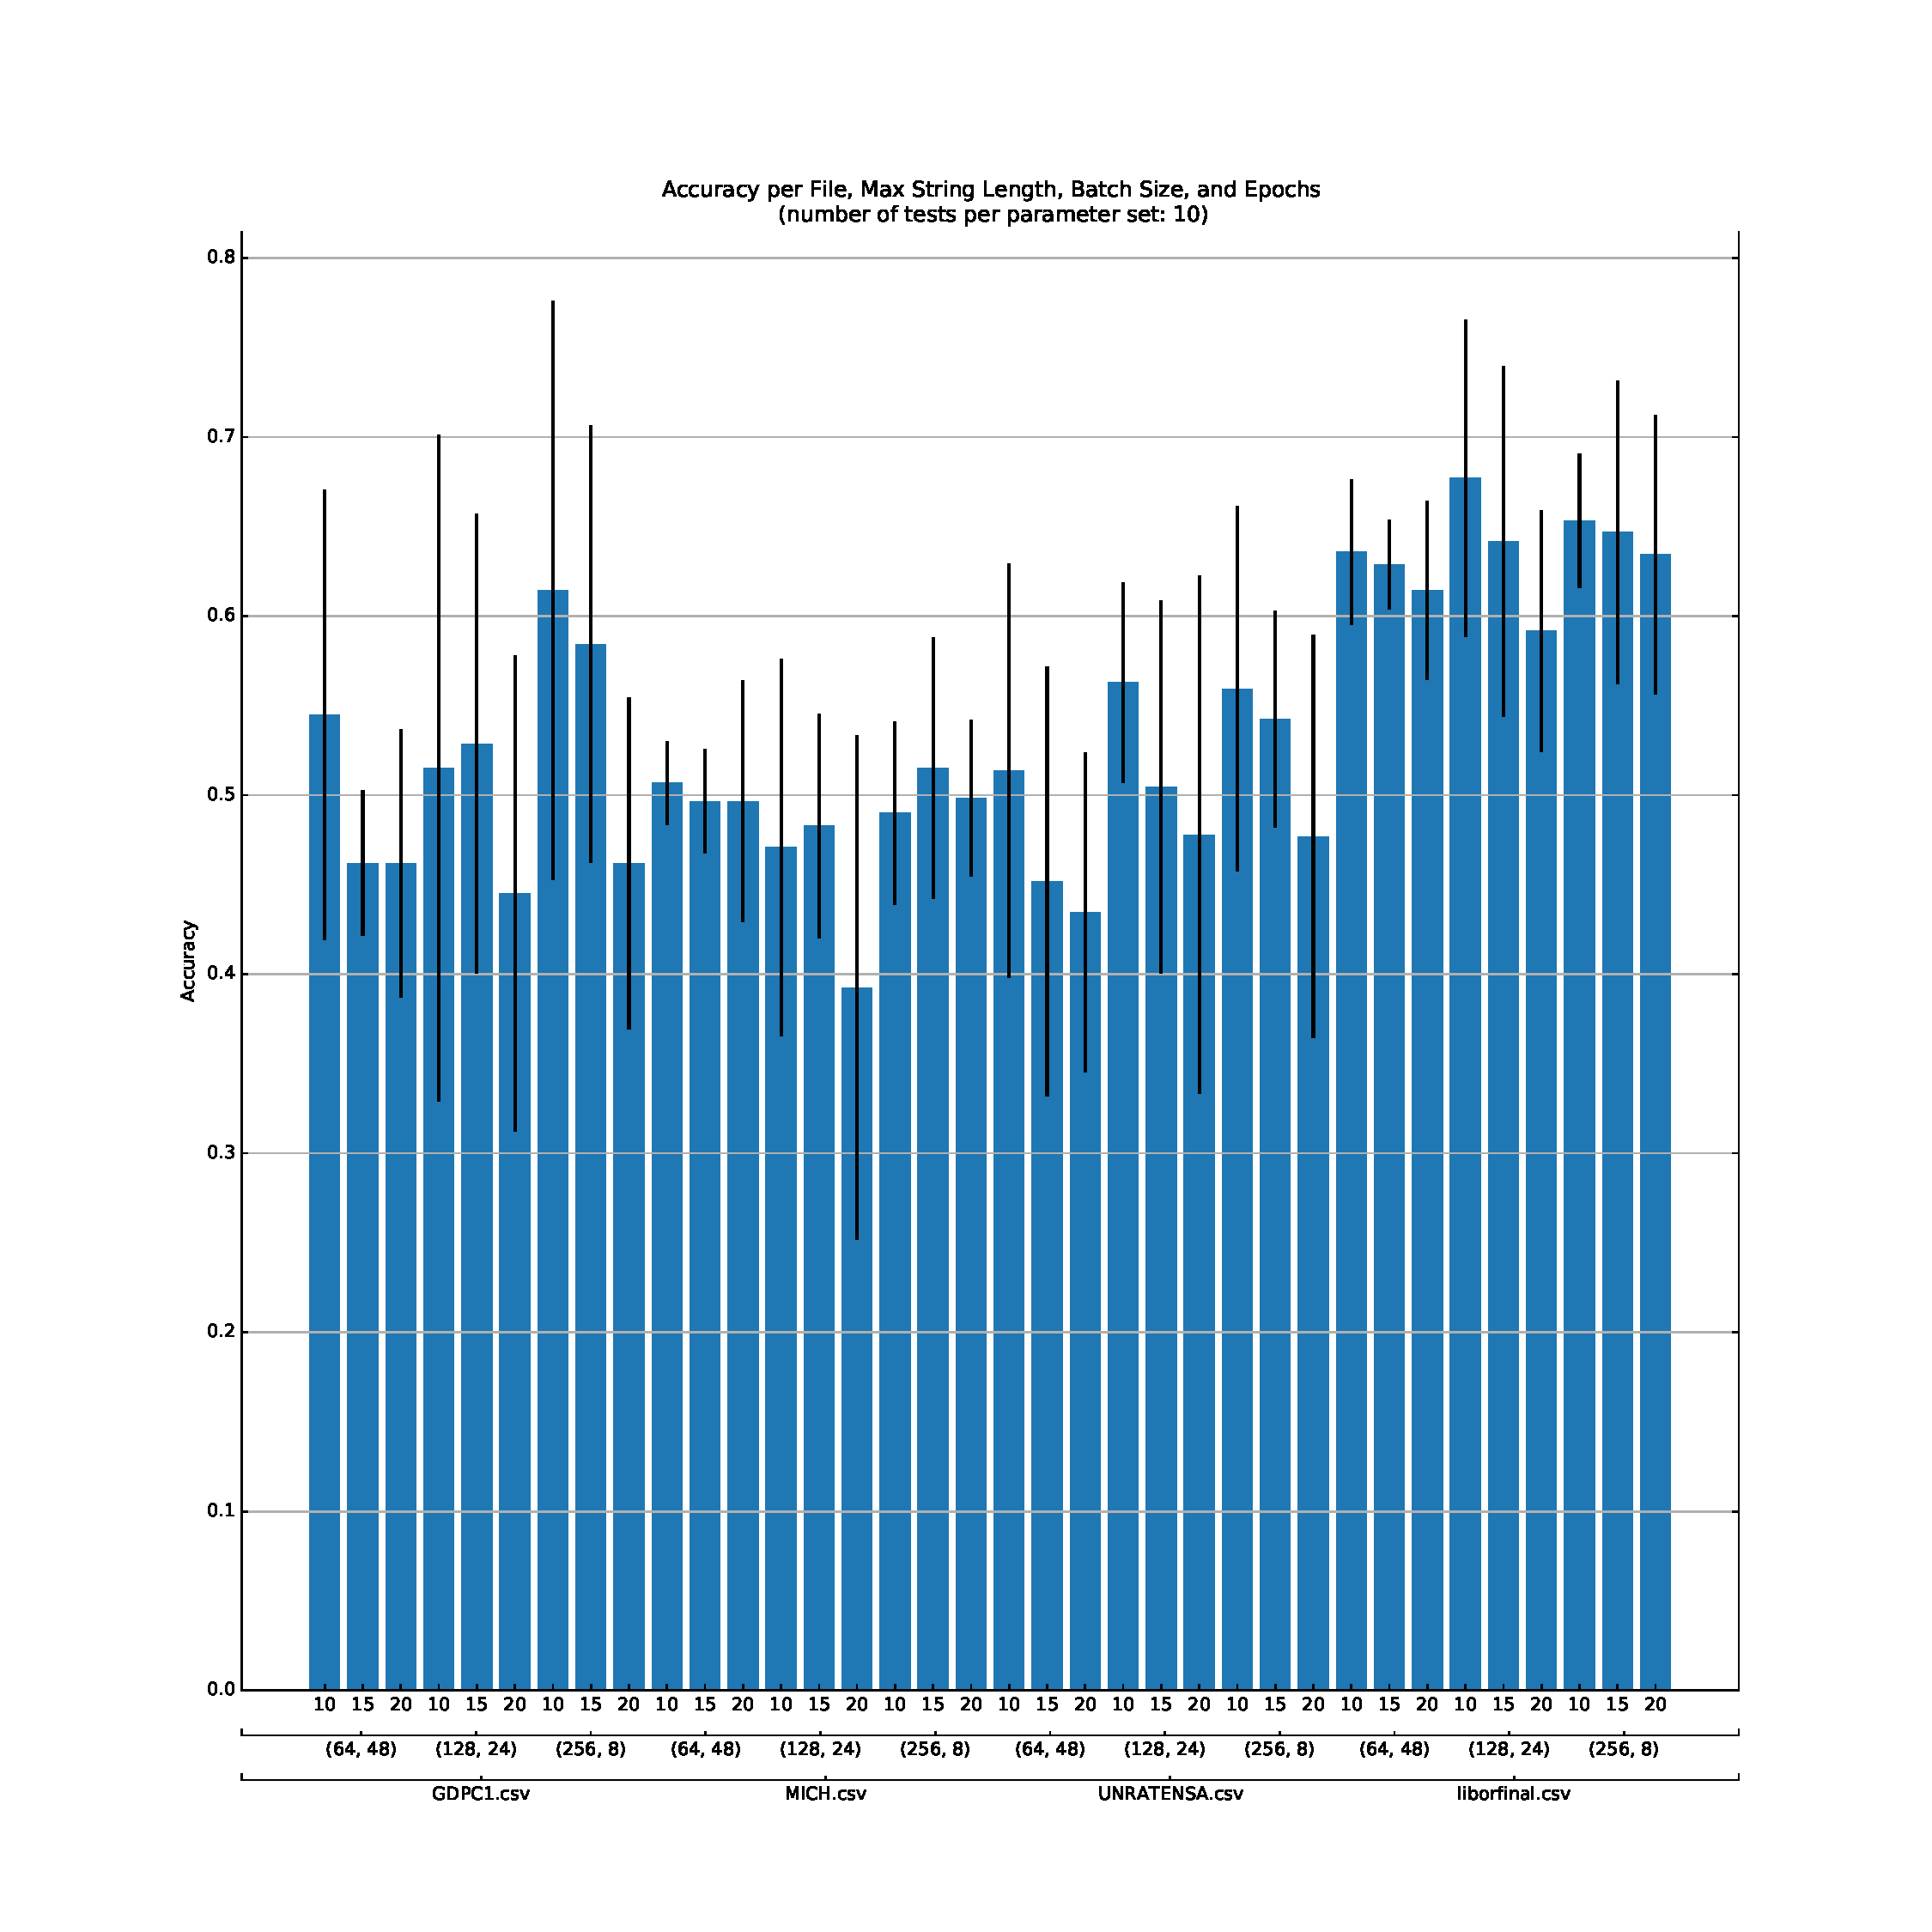
\includegraphics[width=1.03\textwidth,  height=.75\textwidth]{Notes/ParameterSims3.pdf}
    \end{figure}
\end{frame}

\begin{frame}{\XL}
    We see XLNet best predicts Libor Rates just under 70\%.
    Based on these tests, we used the Libor Rates as sentiment with a maximum string length of 256, a batch size of 8, and 10 epochs for training.
\end{frame}

\section{\LS}
\begin{frame}{\LS}
\begin{figure}[htp]
    \centering
    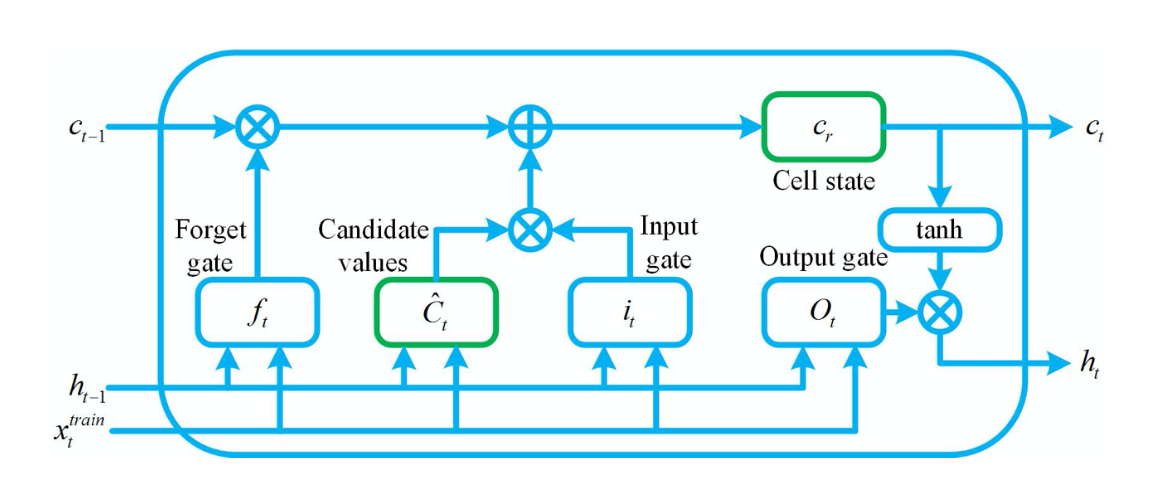
\includegraphics[width=9cm]{LSTM.png}
    \caption{LSTM Procedure}
    \label{fig:LSTM}
\end{figure}
Cell makes decision by considering current input, previous output and previous memory.Generates new output and alters its memory.
\end{frame}




\subsection{\LS}
\begin{frame}{\PRD}
\begin{figure}
\centering
\begin{subfigure}
    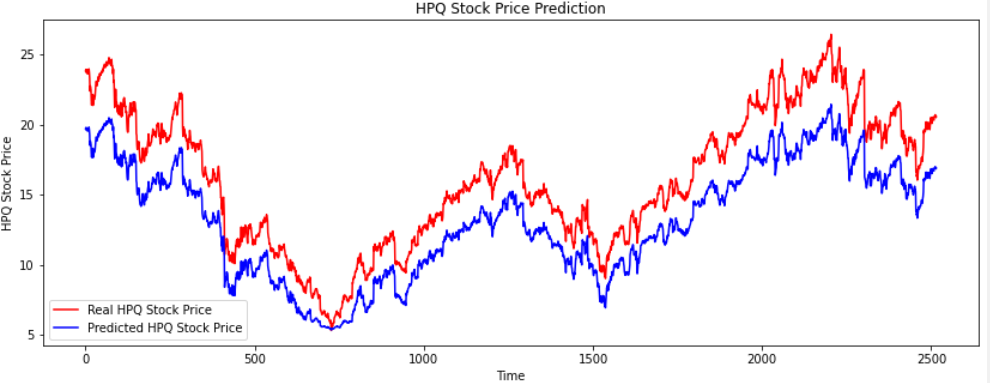
\includegraphics[scale = 0.40]{hpq.png}
    \label{fig:LSTMForecast}
\end{subfigure}
\begin{subfigure}
    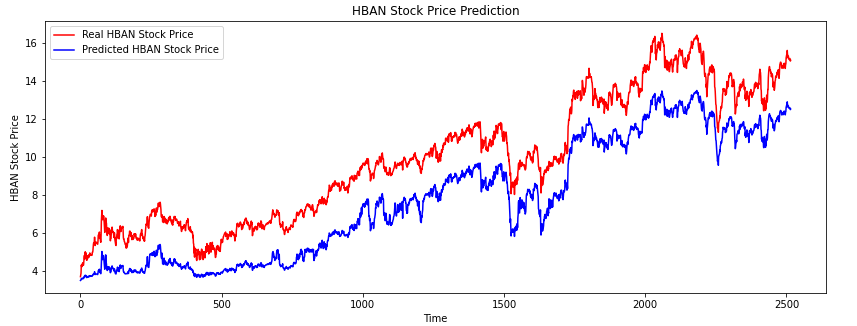
\includegraphics[scale = 0.48]{hban.png}
    \label{fig:LSTMResult}
\end{subfigure}
\end{figure}
\end{frame}

\begin{frame}{\PRD}
\begin{figure}
\centering
\begin{subfigure}
    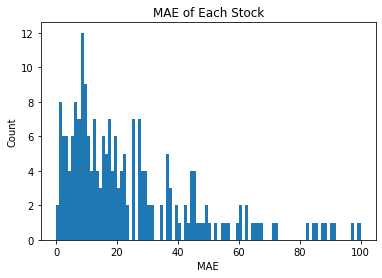
\includegraphics[scale = 0.45]{mae.png}
    \label{fig:LSTMForecast}
\end{subfigure}
\begin{subfigure}
    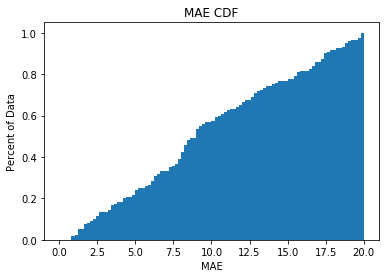
\includegraphics[scale = 0.45]{maecdf.png}
    \label{fig:LSTMResult}
\end{subfigure}
\end{figure}
\end{frame}

\section{\MM}
\begin{frame}{\MM}
    \begin{enumerate}
        \item We first trained the XLNet on the entire text data, and then predicted the sentiment on the same dataset \\
        \item This was then merged with the input data for the LSTM, and was trained using a portion of the stock data \\
        \item Once trained, we validated it with data from 2012 to 2019 and recieved an average error of $62.79$ \\
        \item This is actually worse than our pure LSTM model, indicating our sentiment does not seem to improve our overall model.
    \end{enumerate}
\end{frame}

\section{\CC}
\begin{frame}{\CC}
    \begin{itemize}
        \item We integrated the XLNet models with the LSTM to identify and extract opinions from the federal statement, combining the stock adjust close price and macro-economic data to make stock prediction more accuracy.
        \item The accuracy performance of XLNet-LSTM ends up with an MAE over 60, which is higher than the LSTM MAE of 32. The result means that XLNet can not make the prediction result more accurate and robust.
    \end{itemize}
\end{frame}

\begin{frame}{What's Next}
    \begin{itemize}
        \item Exploding Gradient Problem of LSTM
        \item Market Simulator Plan
        \item Analyze distributions of MAE
    \end{itemize}
\end{frame}{}

\end{document}